% File:  /mit/8.13/presentations/zipped-sample-presentation/sample-presentation.tex
% Updated: June 11, 2008
% Summary: LaTeX template for creating Junior Lab presentations.
%
% Usage: To build a PDF, type `pdflatex sample-presentation.tex'
%        THREE TIMES in order to correct all internal references.
% The Beamer Package Users Guide can be viewed at
% /mit/8.13/presentations/beamerusersguide.pdf
% The users guide is a 224 page document so please don't print it out!

\documentclass[hyperref=pdftex, presentation]{beamer}
% Replacing 'presentation' with 'handout' in the above line
% will produce 4 slides per page.
% The hyperref option makes it possible to include hyperlinks.

\mode<presentation> {
  \usetheme{Boadilla}
  % or CambridgeUS, boxes, Warsaw, Madrid, many others
   %\setbeamercovered{transparent}
  % or whatever (possibly just delete it)
  }

\usepackage[english]{babel}
\usepackage[latin1]{inputenc}
\usepackage{times}
\usepackage[T1]{fontenc}
\usepackage{wrapfig}
\usepackage{graphicx}
\usepackage{adjustbox}
% Or whatever. Note that the encoding and the font should match. If T1
% does not look nice, try deleting the line with the fontenc.

\mode<handout>{
\usepackage{pgfpages}
\pgfpagesuselayout{4 on 1}[a4paper,landscape,border shrink=5mm]
\setbeamercolor{background canvas}{bg=black!10} }

%%%%%%%%%%%%%%%%%%%%%%%%%%%%%%%%%%%%%%%%%%%%%%%%%%%%%%%%%%%%%%%%%%%%%%

\title[Introduction to Magnetars] % (optional)
{Magnetars!}

% \subtitle
% {Presentation Subtitle} % (optional)

\author[Gardner]{Kristen E. Gardner}
\institute[] {UTU - Department of Physics and Astronomy\\}
\date[\today]


% If you wish to uncover everything in a step-wise fashion, uncomment
% the following command:

% \beamerdefaultoverlayspecification{<+->}

% If you wish to uncover everything step by step step just add the command \pause on the specific place.
% Several places are suggested. Just uncomment \pause commands.
% Also- on Organization of talk  [pausesections] as an option.
% Adding the option [handout] to the \documentclass definition will automatically disable all \pause commands
% and will make the frame into slides- in nice printable format.

%;;;;;;;;;;;;;;;;;;;;;;;;;;;;;;;;;;;;;;;;;;;;;;;;;;;;;;;;;;;;;;;;;;;;;;;;;;;;;;;;;;;;;
\begin{document}
\begin{frame}
	\vspace*{-.5cm}
	\begin{center}
		\begin{figure}
			
\includegraphics[scale=.2]{figures/UTU_logo_EN_RGB.png}\hspace*{9cm}
		\end{figure}
	\end{center}
	%\vspace*{-1cm}
  \titlepage
\end{frame}




\begin{frame}{\Large What is a Magnetar?}
\frametitle{\Large What is a Magnetar?}

\begin{minipage}[0.2\textheight]{\textwidth}
\begin{columns}[T]
\begin{column}{0.5\textwidth}

\begin{block}{Definition:}

\begin{itemize}
 \item<2-> neutron star%\pause
 \item<3-> massive magnetic field ($\ge 10^{13}$ G)
\end{itemize}
\end{block}

\end{column}
\begin{column}{0.5\textwidth}
	\begin{figure}
		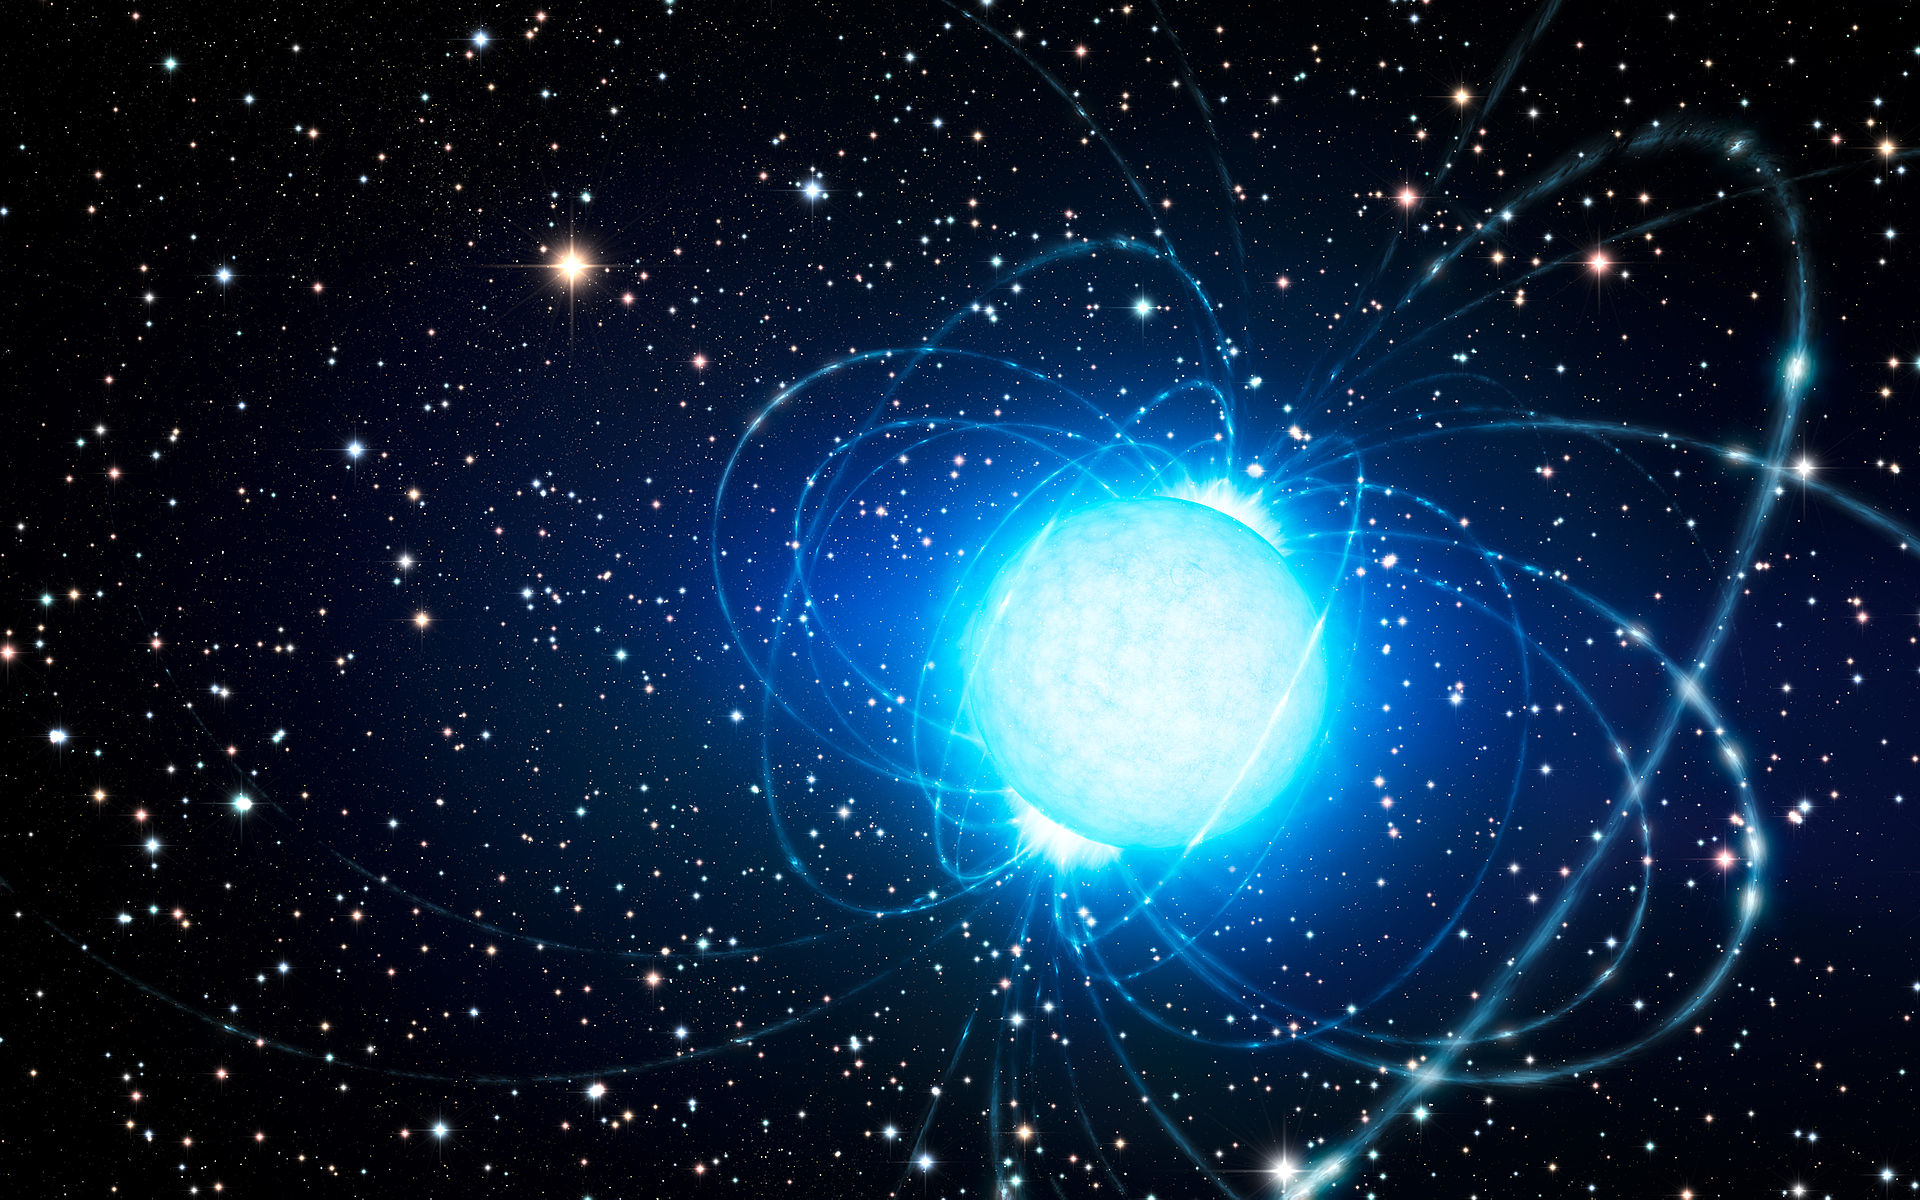
\includegraphics[scale=.09]{figures/magnetar_art.jpg}
		\caption{Artistic depiction of a magnetar}
	\end{figure}
\end{column}
\end{columns}
\end{minipage}

\end{frame}
%;;;;;;;;;;;;;;;;;;;;;;;;;;;;;;;;;;;;;;;;;;;;;;;;;;;;;;;;;;;;;;;;;;;;;;;;;;;;;;;;;;;;;
\begin{frame}{\Large Discovery of Magnetars}
\frametitle{\Large Discovery of Magnetars}

\begin{minipage}[0.2\textheight]{\textwidth}
\begin{columns}[T]
\begin{column}{0.5\textwidth}

\begin{block}{Definition:}

\begin{itemize}
 \item<2-> proposed in 1992 by Duncan Thompson [1]
 \item<3-> SGR 0525-66 found in 1979 (only known outside MW) %European Space Organization's Very Large Telescope
 \item<4-> short X-Ray bursts%\pause
 \item<5-> selection bias 
\end{itemize}
\end{block}

\end{column}
\begin{column}{0.5\textwidth}
	\begin{figure}
		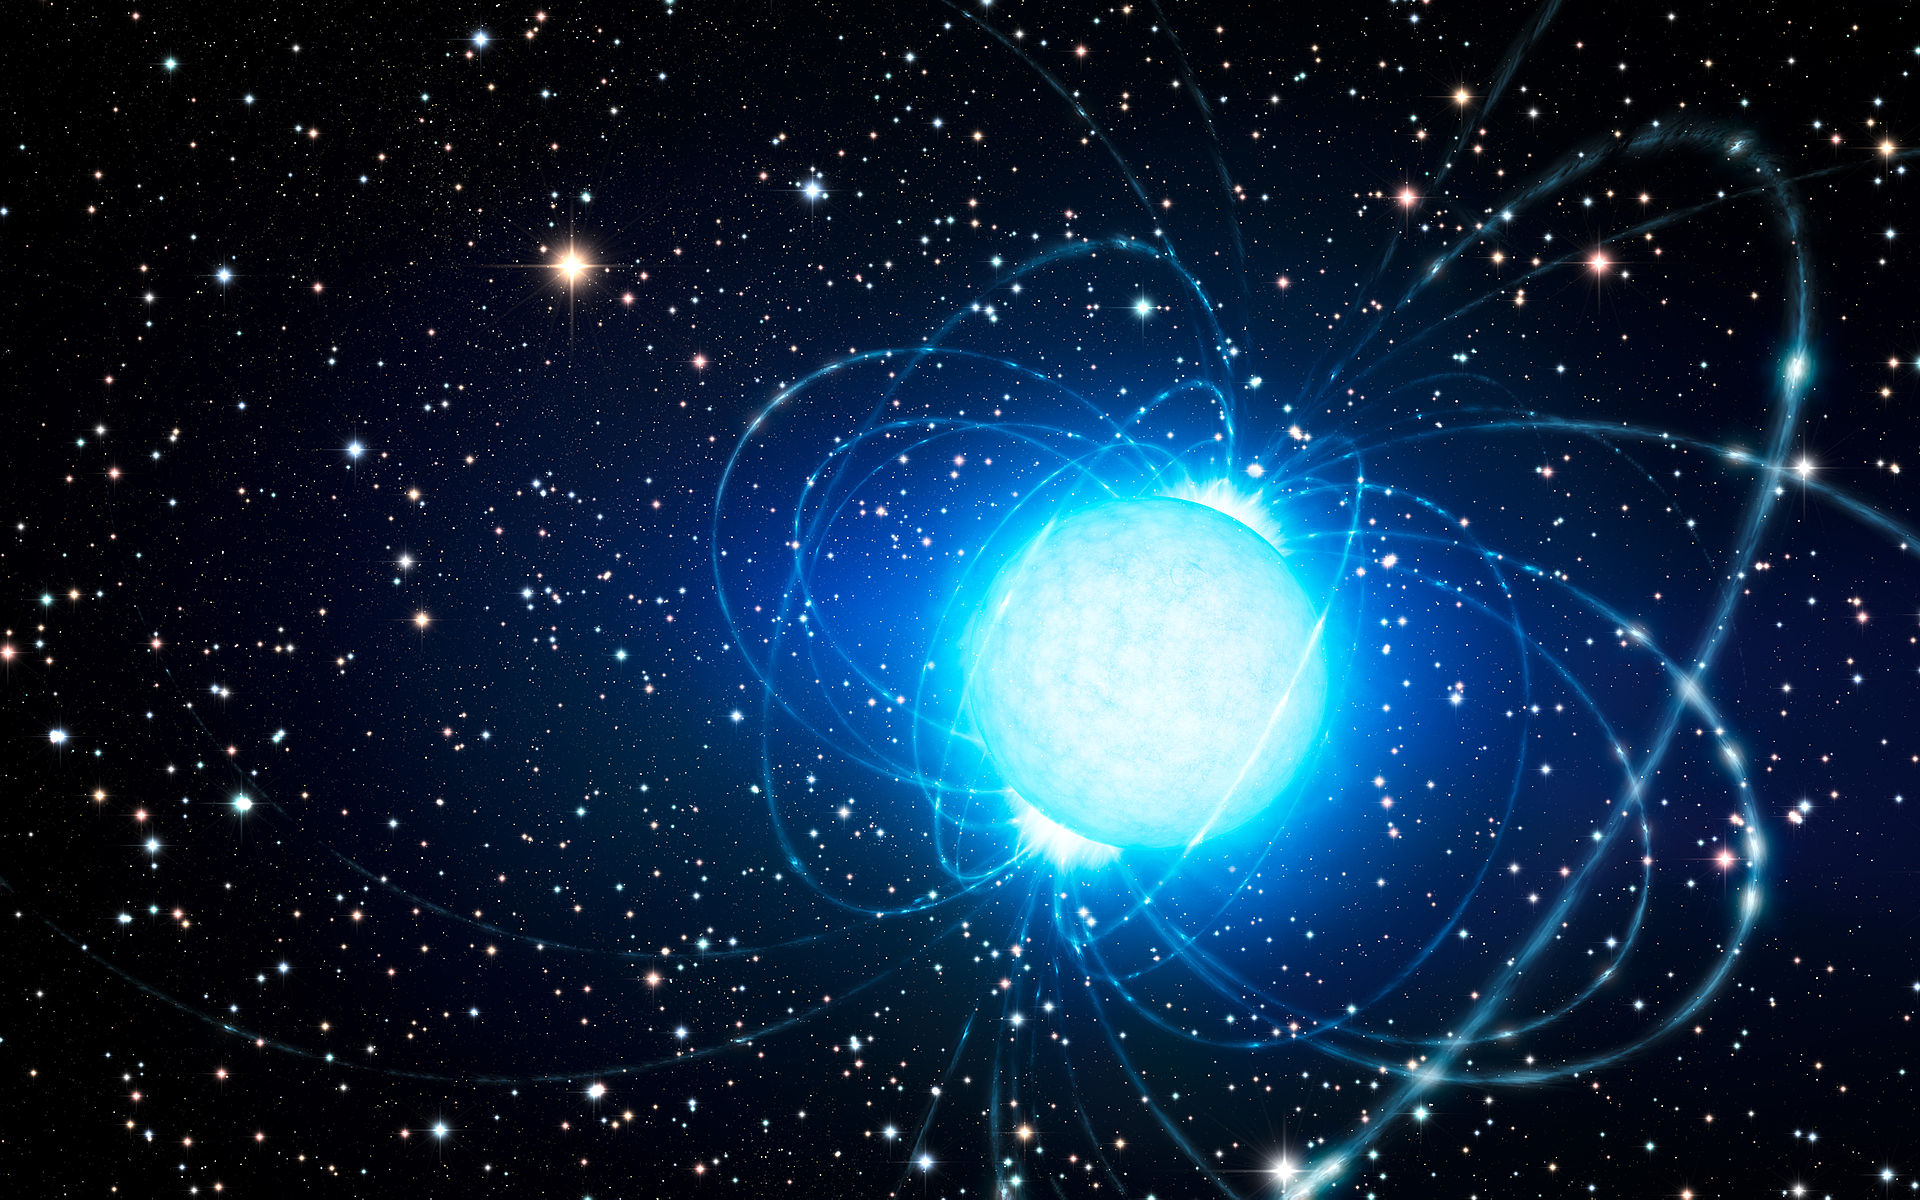
\includegraphics[scale=.09]{figures/magnetar_art.jpg}
		\caption{Artistic depiction of a magnetar}
	\end{figure}
\end{column}
\end{columns}
\end{minipage}

\end{frame}
%;;;;;;;;;;;;;;;;;;;;;;;;;;;;;;;;;;;;;;;;;;;;;;;;;;;;;;;;;;;;;;;;;;;;;;;;;;;;;;;;;;;;;



\begin{frame}{\Large Basic Properties}
\frametitle{\Large Basic Properties}

\begin{minipage}[0.2\textheight]{\textwidth}
\begin{columns}[T]
\begin{column}{0.5\textwidth}

\begin{block}{Description:}

\begin{itemize}
 \item<2-> young neutron star%\pause
 \item<3-> spinning down, timescale $\sim$1 kyr %spinning down without exception, spin-down timescale on the order of thousands of years
 \item<4-> high-B field ($\ge 10^{13}$ G)
 \item<5-> rotational period range of 2-12s %likely due to magnetic breaking
\end{itemize}
\end{block}
\begin{block}{Cases:}

\begin{itemize}
 \item<6-> bi-modal population of transients and persistents%\pause
 \item<7-> cross-species magnetar/pulsar
\end{itemize}
\end{block}
\end{column}
\begin{column}{0.5\textwidth}
	\begin{figure}
		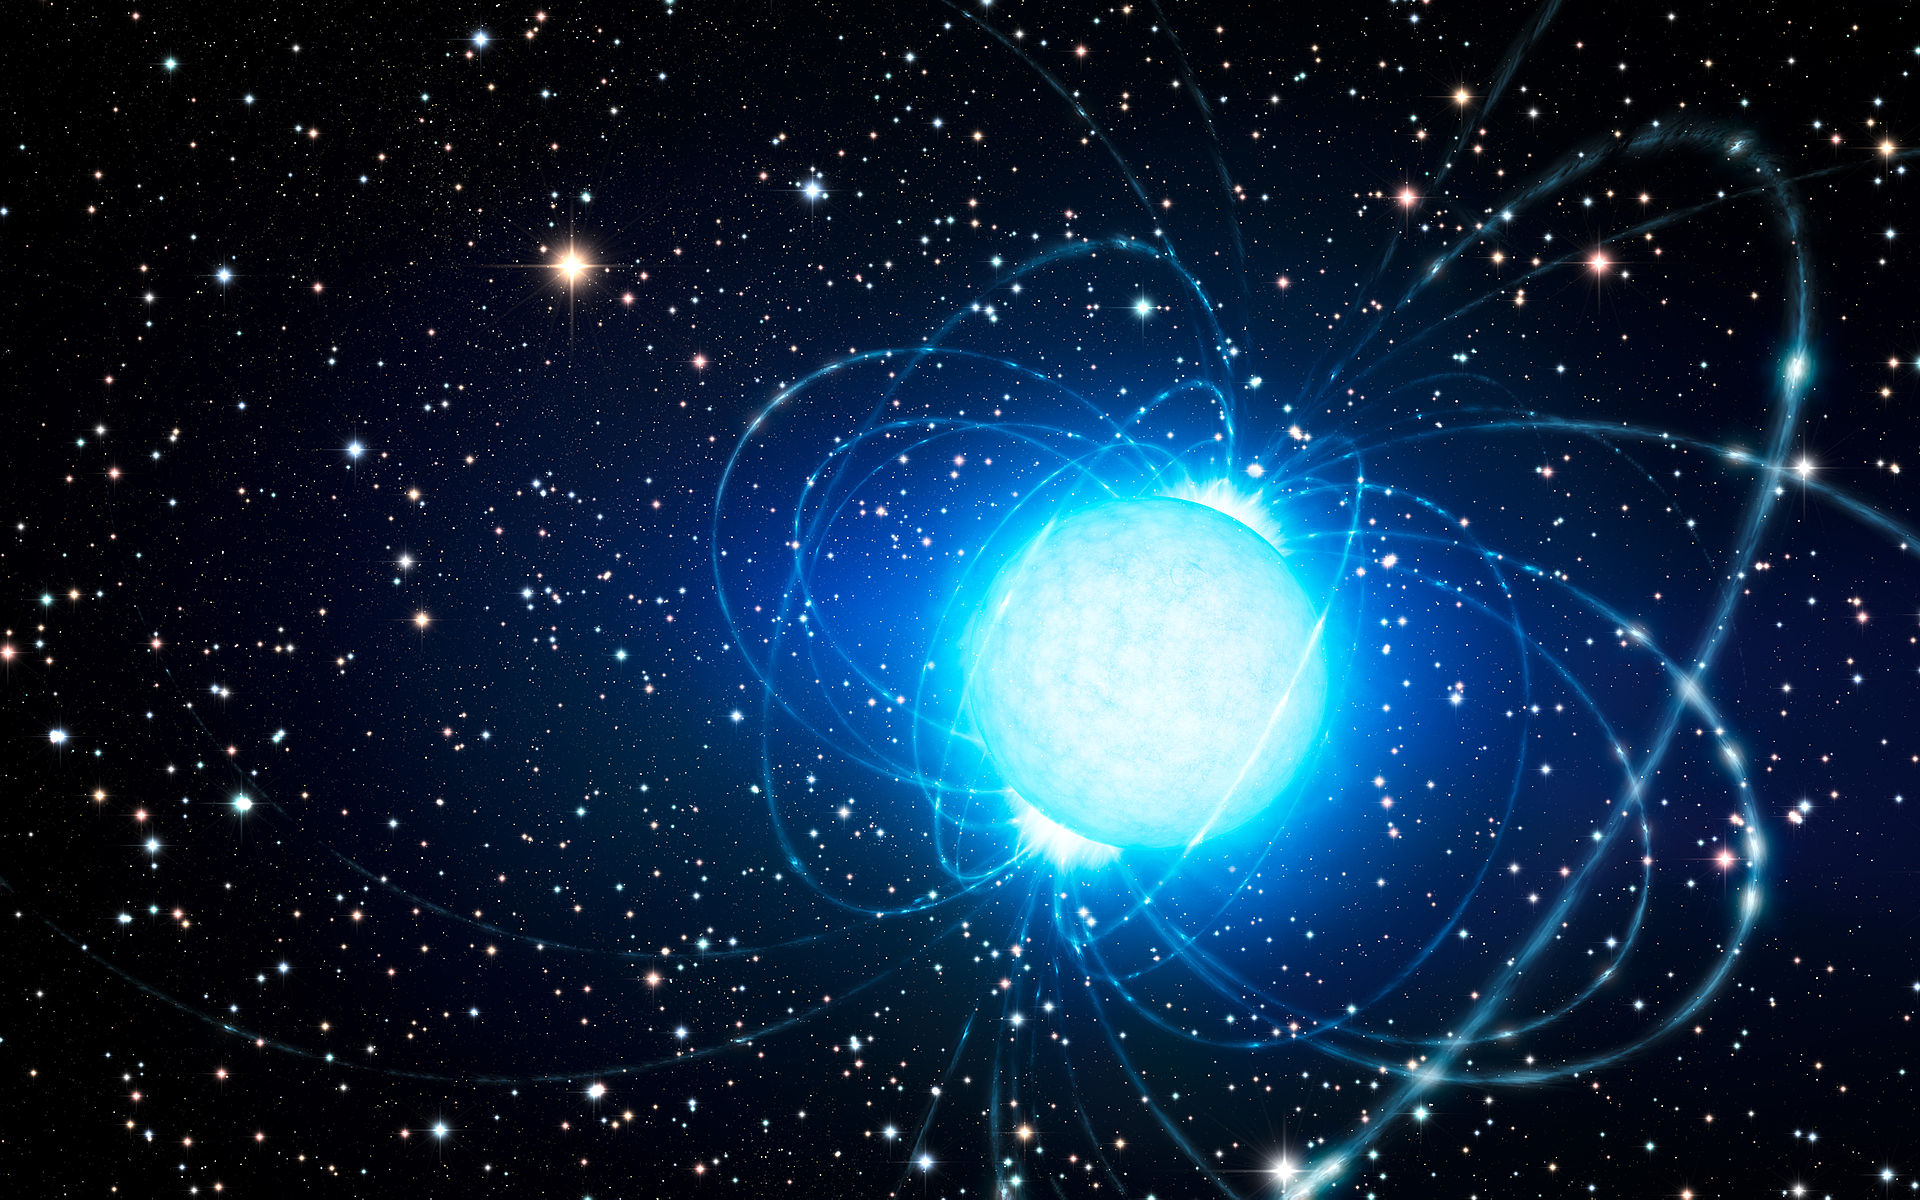
\includegraphics[scale=.09]{figures/magnetar_art.jpg}
		\caption{Artistic depiction of a magnetar}
	\end{figure}
\end{column}
\end{columns}
\end{minipage}

\end{frame}
%;;;;;;;;;;;;;;;;;;;;;;;;;;;;;;;;;;;;;;;;;;;;;;;;;;;;;;;;;;;;;;;;;;;;;;;;;;;;;;;;;;;;;


%columns & blocks: There are two handy environments for structuring
%your slide: "blocks", which divide your slide (horizontally) into
%headed sections, and "columns" which divides your slide (vertically)
%into colum%ns.  This next frame demonstrates both.

\begin{frame}{}
\frametitle{\Large Distinctions}
\begin{columns}[c] % the "c" option specifies center vertical
           % alignment, a `t' option would align the contents
           % top vertically

\column{.7\textwidth} % column designated by a command
\begin{block}{Neutron Star}
\begin{itemize}
 \item radius on order of 10 km%\pause
 \item 1.1 - 2.16 solar masses
 \item $10^9-10^{13}$ G (for non-magnetars)
\end{itemize}
\end{block}
\begin{block}{Magnetars}
\begin{itemize}
 \item<2-> 2-12s rotational period%\pause
 \item<4-> spin-down $\rightarrow$ quiescent X-ray emission and gamma-ray bursts
\end{itemize}
\end{block}
\begin{block}{Radio Pulsars}
\begin{itemize}
	\item<3-> $\sim$100 ms rotational period%period high-band bursts (mostly X-ray)
	\item<5-> spin-down $\rightarrow$ radio emission, and non-thermal X/gamma-ray radiation
\end{itemize}
\end{block}
\column{.3\textwidth}


\end{columns}
\end{frame}




%;;;;;;;;;;;;;;;;;;;;;;;;;;;;;;;;;;;;;;;;;;;;;;;;;;;;;;;;;;;;;;;;;;;;;;;;;;;;;;;;;;;;;

\begin{frame}{\Large Neutron Star Types}
\frametitle{\Large Neutron Star Types}

\begin{figure}
	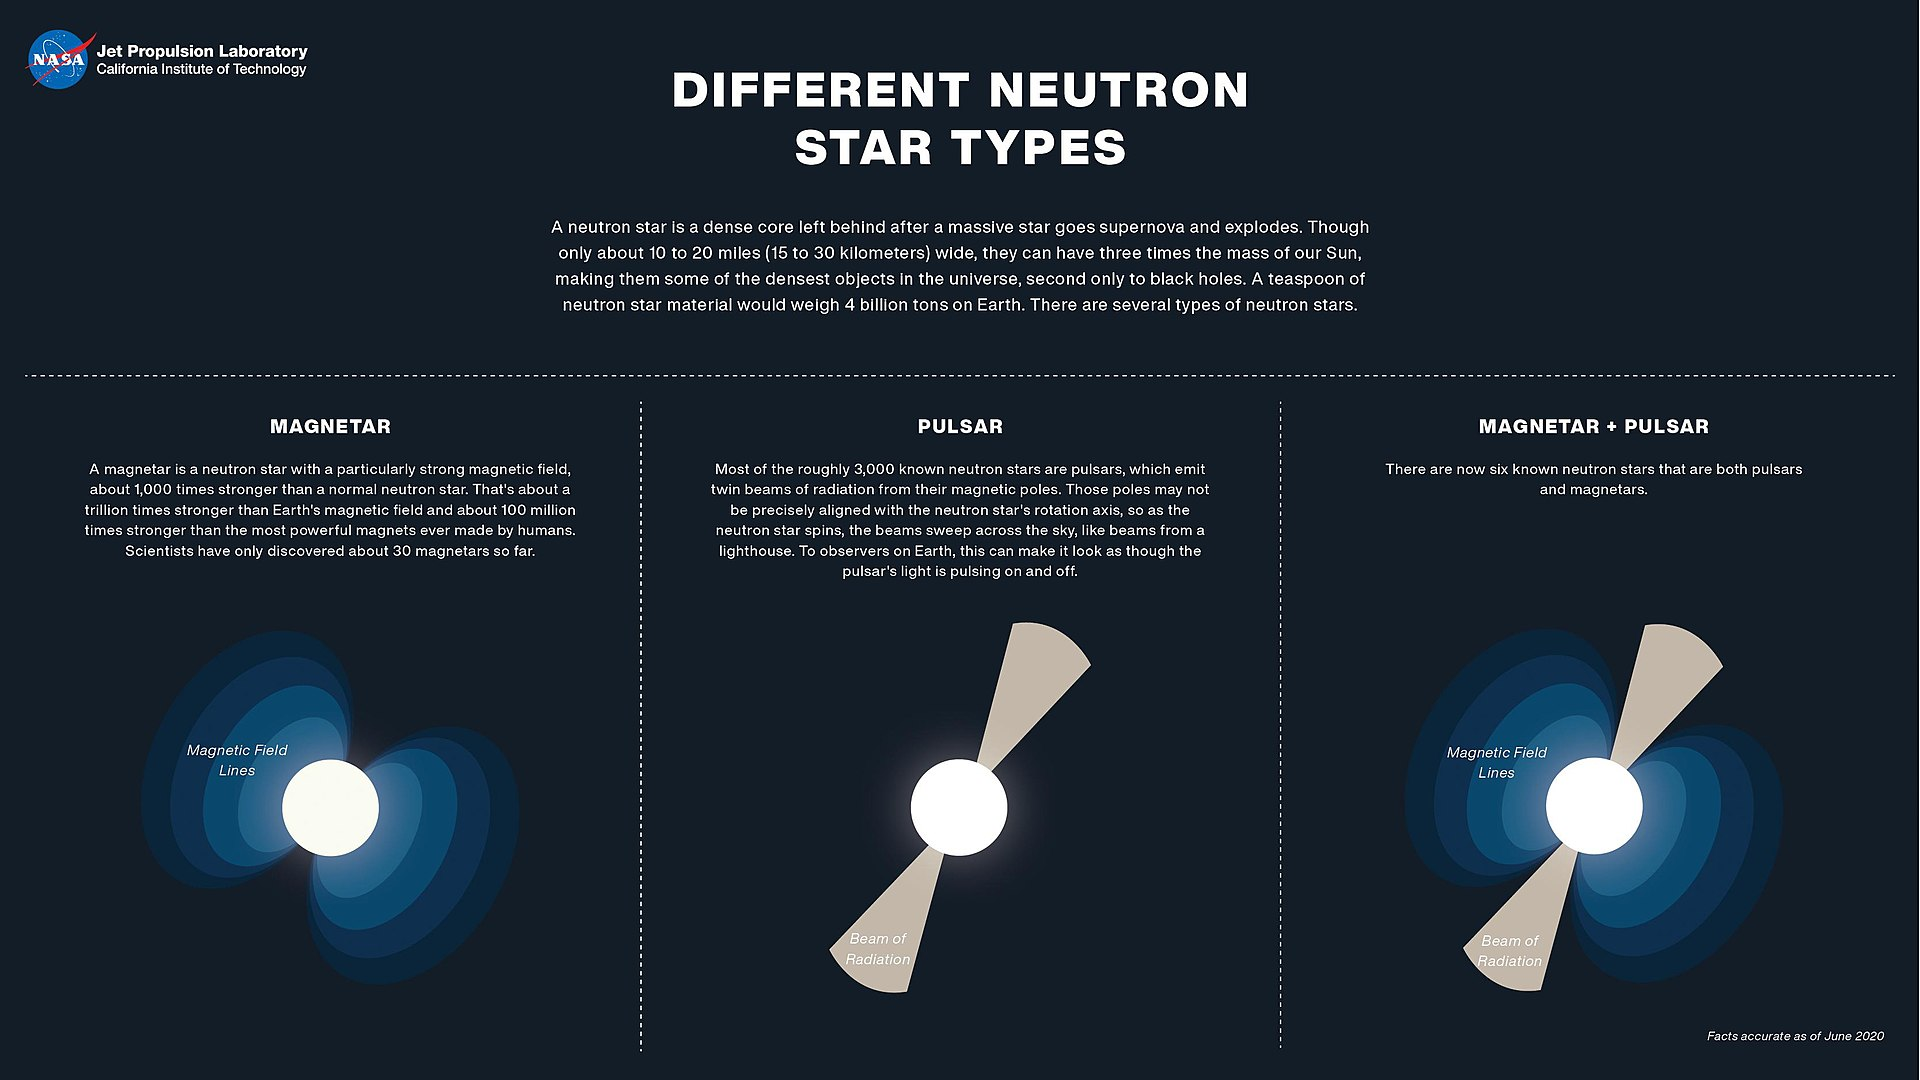
\includegraphics[scale=.17]{figures/neutron_star_types.jpg}
	\caption{Neutron star types, courtesy of JPL [cite here]}
\end{figure}

\end{frame}

%;;;;;;;;;;;;;;;;;;;;;;;;;;;;;;;;;;;;;;;;;;;;;;;;;;;;;;;;;;;;;;;;;;;;;;;;;;;;;;;;;;;;;

\begin{frame}{\Large Distribution in Space}
\frametitle{\Large Distribution in Space}

	\begin{minipage}[0.2\textheight]{\textwidth}
		\begin{columns}[T]
			\begin{column}{0.5\textwidth}
			
				\begin{block}{Observations:}
				
					\begin{itemize}
						 \item<2-> generally within the galactic plane %hence reinforcing the idea of their youth
						 \item<3-> mean speed of 200 km s$^-1$, $\sigma = 100$ km s$^-1$
						 \item<4-> selection bias
					\end{itemize}
				\end{block}
			\end{column}
			\begin{column}{0.5\textwidth}
				\begin{figure}
					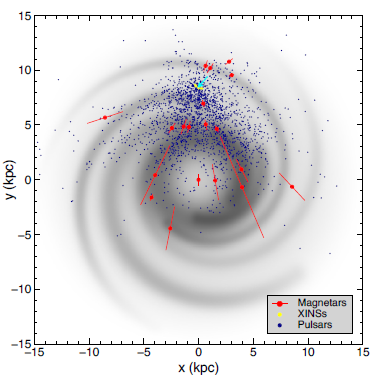
\includegraphics[scale=.5]{figures/spatial.png}
					\caption{Top down view of the Milky Way with known Magnetars (and distance uncertainties) in red.}
				\end{figure}
			\end{column}
		\end{columns}
	\end{minipage}

\end{frame}
%;;;;;;;;;;;;;;;;;;;;;;;;;;;;;;;;;;;;;;;;;;;;;;;;;;;;;;;;;;;;;;;;;;;;;;;;;;;;;;;;;;;;;



\begin{frame}{\Large The Magnetars}
\frametitle{\Large The Magnetars}

\begin{figure}
	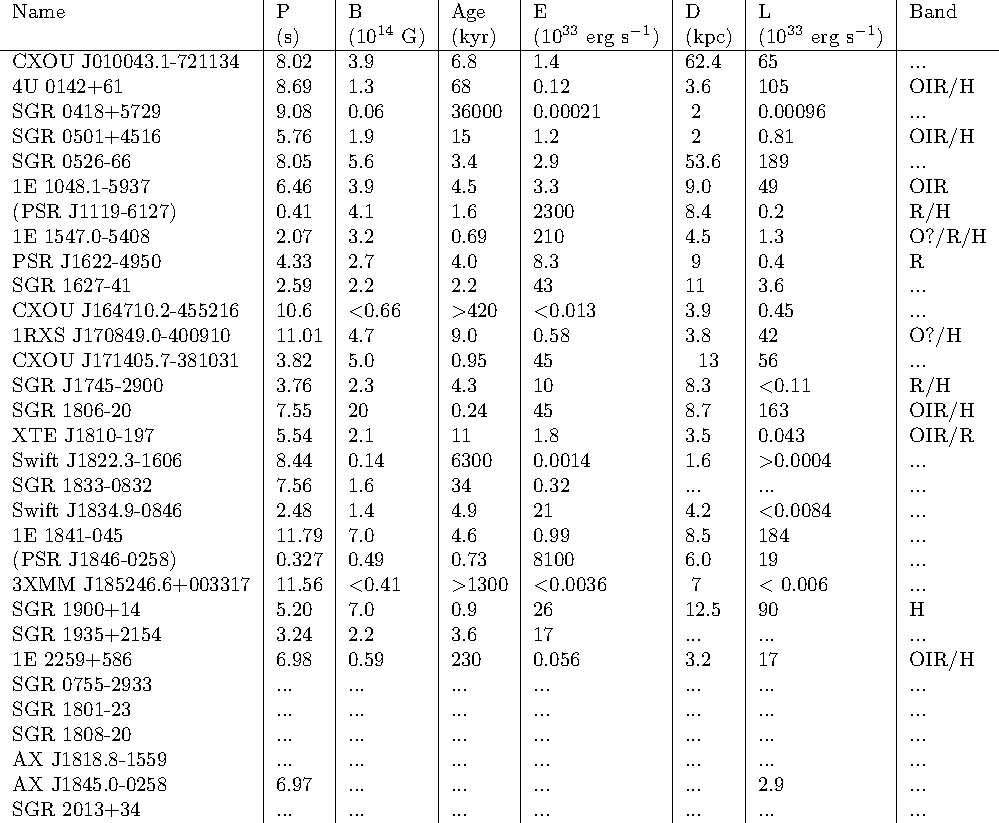
\includegraphics[scale=.5]{tables/magnetar_table.pdf}
	\caption{So far...}
\end{figure}

\end{frame}


%;;;;;;;;;;;;;;;;;;;;;;;;;;;;;;;;;;;;;;;;;;;;;;;;;;;;;;;;;;;;;;


\begin{frame}{\Large Supernova Remnant Associations}
\frametitle{\Large Supernova Remnant Associations}
	
	\begin{minipage}[0.2\textheight]{\textwidth}
		\begin{columns}[T]
			\begin{column}{0.5\textwidth}
			
				\begin{block}{Basics:}
				
					\begin{itemize}
					 \item<2-> 8/23 magnetars  %hence reinforcing the idea of their youth
					 \item<3-> 2 other possible associations
					 \item<4-> provides additional evidence to youth requirement
					\end{itemize}
				\end{block}
				\begin{block}{Consequences:}
				
					\begin{itemize}
					 \item<5-> unexpected characteristics  %hence reinforcing the idea of their youth
					 \item<6-> challenges dynamo model and fossil field theory
					 \item<7-> no conclusive theory of formation as of yet %revise this later
					\end{itemize}
				\end{block}
			\end{column}
			\begin{column}{0.5\textwidth}
				\begin{figure}
					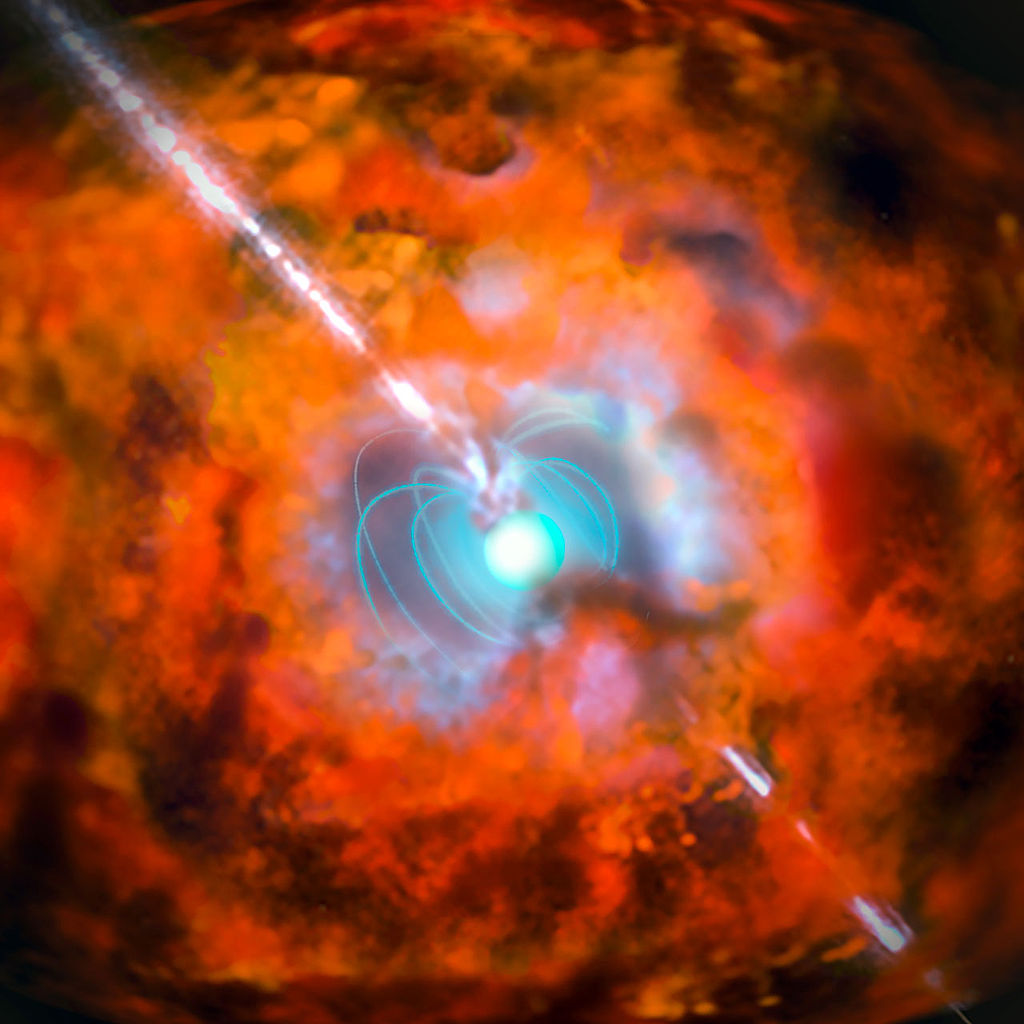
\includegraphics[scale=.15]{figures/magnetar_sn_remnant.jpg}
					\caption{Artist's depiction of supernova remnant and magnetar [Cite here]}
				\end{figure}
			\end{column}
		\end{columns}
	\end{minipage}

\end{frame}

%;;;;;;;;;;;;;;;;;;;;;;;;;;;;;;;;;;;;;;;;;;;;;;;;;;;;;;;;;;;;;
%columns & blocks: There are two handy environments for structuring
%your slide: "blocks", which divide your slide (horizontally) into
%headed sections, and "columns" which divides your slide (vertically)
%into colum%ns.  This next frame demonstrates both.

\begin{frame}{}
\frametitle{\Large Formation}
\begin{columns}[c] % the "c" option specifies center vertical
           % alignment, a `t' option would align the contents
           % top vertically

\column{.7\textwidth} % column designated by a command
\begin{block}{Theories}
\begin{itemize}
 \item<2-> Neutron stars with $\sim$1 ms period at birth [1]%\pause
 \item<4-> Leading Theory: divine entity
\end{itemize}
\end{block}
\begin{block}{Common Conditions}
\begin{itemize}
	\item<3-> parasitic binary star systems ending in supernova %one star feeds on the other, the mass consumption leads to an increase in angular momentum, which - if SN leads to neutron star - allows the neutron star to have the right conditions to be a magnetar
	\item<5-> 
\end{itemize}
\end{block}
\column{.3\textwidth}


\end{columns}
\end{frame}






%;;;;;;;;;;;;;;;;;;;;;;;;;;;;;;;;;;;;;;;;;;;;;;;;;;;;;;;;;;;;;;;;;;;;;;;;;;;;;;;;;;;;;


%columns & blocks: There are two handy environments for structuring
%your slide: "blocks", which divide your slide (horizontally) into
%headed sections, and "columns" which divides your slide (vertically)
%into colum%ns.  This next frame demonstrates both.
\begin{frame}{\Large Kinds of Magnetars}
	\begin{figure}
		\begin{columns}[c] % the "c" option specifies center vertical
           % alignment, a `t' option would align the contents
           % top vertically

			\column{.7\textwidth} % column designated by a command
			\begin{block}{Bi-modal}
				\begin{itemize}
					\item<2-> Persistent Magnetars
					\item<3-> Transient Magnetars
				\end{itemize}
			\end{block}
			\begin{block}{Cross-species}
				\begin{itemize}
 					\item<4-> Magnetar Pulsar%\pause
 					\item<5-> Theoretically: neutron star switch between magnetar, pulsar, and magnetar pulsar
				\end{itemize}
			\end{block}
			
			\column{.3\textwidth}

		\end{columns}
	\end{figure}
\end{frame}


\begin{frame}{\Large Magnetic Breaking}
	\begin{figure}
		\begin{columns}[c] % the "c" option specifies center vertical
           % alignment, a `t' option would align the contents
           % top vertically
			
			\column{.7\textwidth} % column designated by a command
			\begin{block}{Materials}
				\begin{itemize}
 					\item<2-> 
				\end{itemize}
			\end{block}
			
			\column{.3\textwidth}
		\end{columns}
	\end{figure}
\end{frame}


\begin{frame}{\Large EM-Bursts}
	\begin{figure}
		\begin{columns}[c] % the "c" option specifies center vertical
           % alignment, a `t' option would align the contents
           % top vertically
			
			\column{.7\textwidth} % column designated by a command
			\begin{itemize}
				\item<2->
			\end{itemize}
			
			\column{.3\textwidth}
		\end{columns}
	\end{figure}
\end{frame}



%;;;;;;;;;;;;;;;;;;;;;;;;;;;;;;;;;;;;;;;;;;;;;;;;;;;;;;;;;;;;;;;;;;;;;;;;;;;;;;;;;;;;;



%;;;;;;;;;;;;;;;;;;;;;;;;;;;;;;;;;;;;;;;;;;;;;;;;;;;;;;;;;;;;;;;;;;;;;;;;;;;;;;;;;;;;;
\begin{frame}{Summary and Conclusions}

  % Keep the summary *very short*.
  \begin{columns}[c] % the "c" option specifies center vertical
           % alignment, a `t' option would align the contents
           % top vertically

			\column{.7\textwidth} % column designated by a command
			\begin{block}{What we know}
				\begin{itemize}
 					\item<2-> 
				\end{itemize}
			\end{block}
			\begin{block}{What we don't know}
				\begin{itemize}
 					\item<3-> A definitive model for the formation of magnetars %we need to observe more. Given their short life times, it will take a large scale operation to observe enough to build a more robust model of how they form and the related mechanics of them.
				\end{itemize}
			\end{block}
			\column{.3\textwidth}

		\end{columns}
\end{frame}


\begin{frame}{References}
	\begin{enumerate}
		\item Duncan RC, Thompson C. 1992. ApJ 392:L9-L13
	\end{enumerate}
\end{frame}

\end{document}
